\documentclass{article}
\usepackage[letterpaper]{geometry}
\geometry{verbose,tmargin=1in,bmargin=1in,lmargin=1in,rmargin=1in}

\usepackage[utf8]{inputenc}
\usepackage{amsmath}
\usepackage{listings}
\usepackage{graphicx}
\usepackage{enumitem}

\title{CIS 419/519: Homework 1}
\author{Jiatong Sun}
\date{}

\begin{document}
    \maketitle
    Although the solutions are entirely my own, I consulted with the following people and sources while working on this homework: Yupeng Li, Maian Zhang, Yuchen Sun, Jianshu Hu, https://pandas.pydata.org/pandas-docs/stable/
    
    \section{Decision Tree Learning}
        \begin{enumerate}[label=\alph*.]
            \item % a
            Show your work:
            \begin{equation*}
            	\begin{split}
                &\mathit{InfoGain}(\mathit{PainLocation})\\
                =\quad&\mathit{Info(X)-Info(X|			
                PainLocation)}\\
                =\quad&[-(\frac{9}{14}\log_2\frac{9}{14}+
                \frac{5}{14}\log_2\frac{5}{14})]\\
                \quad&-\left\{-[\frac{5}{14}
                (\frac{3}{5}\log_2\frac{3}{5}+
                \frac{2}{5}\log_2\frac{2}{5})+
                \frac{5}{14}
                (\frac{2}{5}\log_2\frac{2}{5}+
                \frac{3}{5}\log_2\frac{3}{5})+0
                ]\right\}\\
                =\quad&0.9402-0.6935\quad
                =\quad0.2467\\\\
                &\mathit{InfoGain}(\mathit{Temperature})\\
                =\quad&mathit{Info(X)
                -Info(X|Temperature)}\\
                =\quad&[-(\frac{9}{14}\log_2\frac{9}{14}+
                \frac{5}{14}\log_2\frac{5}{14})]\\
                \quad&-\left\{-[\frac{10}{14}
                (\frac{3}{10}\log_2\frac{3}{10}+
                \frac{7}{10}\log_2\frac{7}{10})+
                \frac{4}{14}
                (\frac{2}{4}\log_2\frac{2}{4}+
                \frac{2}{4}\log_2\frac{2}{4})+0
                ]\right\}\\
                =\quad&0.9402-0.9152\quad
                =\quad0.0250
                \end{split}
            \end{equation*}
            
            \item % b
            Show your work:
            \begin{equation*}
            	\begin{split}
                &\mathit{GainRatio}(\mathit{PainLocation})
                \\=\quad&\mathit{
                \frac{InfoGain(PainLocation)}
                {SplitInformation(PainLocation)}}\\
                =\quad&0.2467\div\left\{-[
                \frac{5}{14}\log_2\frac{5}{14}+
                \frac{5}{14}\log_2\frac{5}{14}+
                \frac{4}{14}\log_2\frac{4}{14}]\right\}\\
                =\quad&0.2467\div1.5774\quad
                =\quad0.1564\\\\
                &\mathit{GainRatio}(\mathit{Temperature}) =
                \\=\quad&\mathit{
                \frac{InfoGain(Temperature)}
                {SplitInformation(Temperature)}}\\
                =\quad&0.0250\div\left\{-[
                \frac{10}{14}\log_2\frac{10}{14}+
                \frac{4}{14}\log_2\frac{4}{14}]\right\}\\
                =\quad&0.2467\div0.8361\quad
                =\quad0.2950
                \end{split}
            \end{equation*}
            
            \item % c 
			\begin{figure}[h]
			\centering
			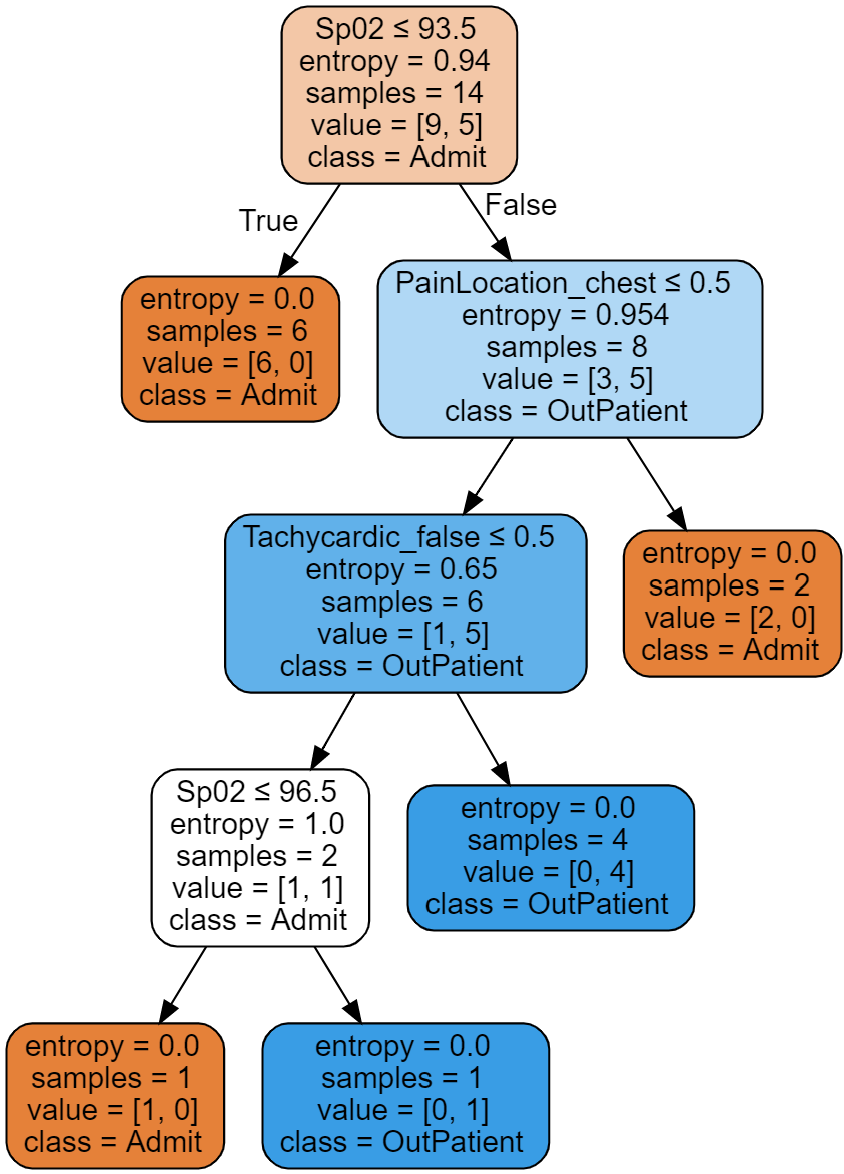
\includegraphics[width=0.5\textwidth]
            {UnprunedTree.png}
            \caption{Unpruned Tree}
            \label{fig:PrunedTree}
			\end{figure}
            
                     
            \item % d
            No because finding the global optimal decision 
            tree is an NP-Complete problem, whereas ID3
            utilizes a greedy approach to select the
            locally best attribute to split the dataset.\\
            \\The advantage of ID3 is that it works really
            fast and usually produces a relatively small
            tree, though not the smallest.
        \end{enumerate}
        
       \section{Decision Trees \& Linear Discriminants [CIS 519 ONLY]}
        
        A decision tree can include oblique splits by using  a weighted average of different features. \\\\
        The definition of "a split parallel to an axis" means for each feature after preprocessing (after converging to binary and OHE), a split on any feature becomes a threshold, which is demonstrated as a line perpendicular to this feature on the visualized coordinate system. In this way, this line can defined as parallel to other feature axis.\\\\
        There does exist a way to generate an obique split. For example, if two features (A, B) are considered in the training set, then a classical decision tree will result in a split parallel to x axis or y axis. However, we can use C = kA + (1-k)B to represent this feature, where k is a real number between 0 and 1 (0 and 1 not included). In this way, the new split is only related to feature C and we can assume the split is at C = kA + (1-k)B = m. This equation is actually an expression of a line in A-B plane, which is not parallel to either axis.
        
        
        \section{Programming Exercises}
        \textbf{Features}: What features did you choose and how did you preprocess them?\\\\
        The preprocessing consists of the following two procedures.
        \begin{itemize}
        \item[1.]Delete columns whose missing ratio is too high. \\
        Here I set the missing ratio threshold to 0.6, which means if a column lacks more than sixty percent data, this column will be removed.
        \item[2.]Replenish NaN in the remaining data set.\\ 
        For numerical features, I use the mean value of each column to fill the NaN.\\
        For category features, I use the mode of each column to fill the NaN and then use one-hot-encode method to split mutiple-value features into several binary features.
        \end{itemize}
        There are three sets of features that I chose, each one derived from a distinct method.
        \begin{itemize}
        	\item[1.]Using \textbf{Pandas.DataFrame.corr} function, which computes pairwise correlation of columns excluding NA/null values. By computing the correlation parameters between each feature column and y, then sort their absolute values descendingly. Keep the top 13 features as the first feature set.
        	\item[2.]Using \textbf{Python Random shuffle()} to select 13 features randomly to form a feature set.
        	\item[3.]Using the features included in the online example. The Glycohemoglobin A1C feature should be deleted here according to the requirement. So the third feature set also consists of 13 features.
        \end{itemize}
        After calculating the average cross-validation accuracy over three different data set, the best feature set is the first one, which utilizes correlation parameter method. The selected best feature set is listed below.\\
        \begin{center}
        	\begin{tabular}{|c|c|c|c|}
        		\hline
        		'LBDSGLSI'&'LBXSGL'&'DIQ050'&'RIDAGEYR'\\
        		\hline
        		'BMXWAIST'&'BMDAVSAD'&'BMXSAD2'&'BMXSAD1'\\
        		\hline
        		'DMDHHSZE'&'HUQ010'&'DMDHRAGE'&'BPQ090D'\\
        		\hline
        		'BMXBMI'&&&\\
        		\hline
        	
        	\end{tabular}
        	
        \end{center}
		
		
		As is shown below, the final pruned tree has only one root and two leaves. The only used feature is 'LBDSGLSI', which stands for Glucose (mmol/L)        
        
        \begin{figure}[h!]
       	\centering
		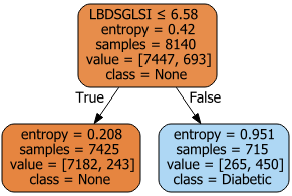
\includegraphics[scale=2]{PrunedTree.png}
  		\caption{Pruned Tree}
  		\label{fig:PrunedTree}
		\end{figure}        
        
        \newpage                     
        \noindent\textbf{Parameters}: What parameters did you use to train your best decision tree\\\\
        After several experiment, I notice the accuracy remains a highest constant on a relatively long interval, normally (0.01,0.20) with respect to \texttt{ccp\_alpha}. The interval range varies slightly according to the different parameters used in the preprocess. Following this regulat pattern, I calculate the cross-validation accuracy with an ascending \texttt{ccp\_alpha} value and confirm the best value once the accuracy starts to drop. In my current program, the best \texttt{ccp\_alpha} is computed to be approximately 0.14.\\\\

        \noindent\textbf{Performance Table}: 
        \begin{center}
            \begin{tabular}{|c|c|c|}
                \hline
                Feature Set & Accuracy & Conf. Interval [519 ONLY]\\
                \hline
                DT 1 & 0.929 & (0.927,0.931)  \\
                DT 2 & 0.865 & (0.863,0.868)  \\
                DT 3 & 0.878 & (0.875,0.881)  \\
                \hline
        \end{tabular}
                \end{center}
        
        
        
        \textbf{Conclusion}: What can you conclude from your experience?\\
        \begin{itemize}
        	\item[1.]Within a large data set, there are only several key features that exert the most crucial influence on the model, so it's important to properly preprocess the data set. At the same time, a good preprocessing also significantly reduces the time of machine learning.
        	\item[2.]Correlation method is useful to select important features. It does obviously better job than a random feature set.
        	\item[3.]Pruning is beneficial to making a decision tree. Tuning the \texttt{ccp\_alpha} can increase the accuracy and simplify the model by decreasing the tree's depth.
        	\item[4.]Cross-Validation is a good way to take advantage of more data. It not only prevents an extreme occasionality, but doesn't have a too high cost of time as well. Its average accuracy, however, is not fixed but constriced to a range, which can be estimated by Student's t-distribution.
        \end{itemize}
        
\end{document}